%\documentclass[11pt]{book}
\documentclass[10pt]{article}
%\documentclass[11pt]{amsart}
%\documentclass[preprint,12pt]{elsarticle}
\usepackage{multirow}
\usepackage[all]{xy}
\usepackage{verbatim} 
\usepackage{endnotes}
\usepackage{amssymb} 
\usepackage{setspace} 
%\doublespacing
\onehalfspacing
%\usepackage{mathabx}
\usepackage{amsmath}
\usepackage{hyperref} % for urls
\hypersetup{pdfborder={0 0 0}}

%\usepackage{diagrams}

%\usepackage{bookman}
%\usepackage{helvet}
\usepackage{palatino}
%\usepackage{times}


%\usepackage{charter}
%\usepackage{avant}
%\usepackage{chancery}
%\usepackage{utopia}

\def\setgrouptext#1{\gdef\grouptext{#1}}
\newenvironment{groupeditems}{\begin{displaymath}\left.\vbox\bgroup\setgrouptext}{%
  \egroup\right\rbrace\hbox{\grouptext}\end{displaymath}}
  
\usepackage{fancyhdr}

%\pagestyle{fancy}

\usepackage{sectsty}
%\allsectionsfont{\sffamily} 
\chapterfont{\Large \scshape}
\sectionfont{\large \scshape \centering}
\subsectionfont{\normalsize \itshape}
%\subsectionfont{\large \nohang \flushleft} 
%\allsectionsfont{\mdseries\itshape} 
%\sectionfont{\fontfamily{ptm}\selectfont}

% \usepackage{fullpage}


\usepackage[margin=1.5in]{geometry}

\usepackage{lastpage}

\usepackage{fancyhdr}
\setlength{\headheight}{15.2pt}
\pagestyle{fancy}

%\rhead[<even output>]{\textsc{\large Dissertation Summary} --  \thepage \textit{ of}   \pageref{LastPage}}
\rhead[<even output>]{\textsc{\small Evidential Reasoning} -- \ \thepage \textit{ of}   \pageref{LastPage}}
%\chead[<even output>]{<odd output>}
\lhead[<even output>]{\text{\small Di Bello \& Verheij}}

%\lfoot[<even output>]{<odd output>}
\cfoot[<even output>]{}
%\rfoot[<even output>]{ \thepage \textit{ of}   \pageref{LastPage}}




\usepackage{pgfplots}

 
\usepackage[round]{natbib}
\begin{document}

\thispagestyle{empty}

\vspace{-2cm}
\noindent
%\section*{ \hspace{6cm} \Large DRAFT - begin}
-----------------------------------------------------------------------------------------------------------------------
%\section*{ \Large Writing Sample A}


\vspace{5mm}
\noindent
\textsc{\large \bf  EVIDENTIAL REASONING \\ Chapter for the Handbook of Legal Reasoning}

\vspace{3mm}
\noindent
Marcello Di Bello \& Bart Verheij --  \today \\
%Word count:  9723.
\vspace{1cm}

\vspace{1cm}



\vspace{1cm}

%\begin{abstract}
%mmm
%\end{abstract}

%QUESTION: WILL THIS BE A "US CENTRIC" CHAPTER? I HATE THAT, BUT I AM AFRAID MY PART WILL BE US CENTRIC. 

\tableofcontents

\newpage

\noindent When a suspect appears in front of a criminal court, there is a very high probability that he will be found guilty. In the Netherlands, for instance, the conviction rate of suspects that appear in criminal courts is reported to be around 95\% year after year.\footnote{Source: CBS, the Dutch central bureau of statistics, publishing its data at www.cbs.nl.} In the United States, the conviction rate in federal courts has been roughly 75\% and in Japan it has reached as high a rate as 99\%.\footnote{\textbf{SOURCE TO BE ADDED}} This does not mean that fact-finders deciding about the facts of a criminal case have an easy job. Whether laypeople, such as jury members selected from the general public, or professionals, often experienced judges having completed postgraduate education, all face the difficulties associated with handling the evidence that is presented in court. What to do with conflicting testimonies? Does an established DNA match outweigh the testimony that the suspect was not on the crime scene? How to coherently interpret a large body of evidence? What to do with illegally obtained evidence? When is there enough evidence to convict `beyond a reasonable doubt'? 

The primary aim of this chapter is to explain the nature of evidential reasoning, the characteristic difficulties encountered, and the tools to address these difficulties. There is an extensive scholarly literature on these topics, and it is a secondary aim of the chapter to provide readers the means to find their way in historical and ongoing debates. Before diving into the literature, we set the stage by using two important and often encountered kinds of evidence as an illustration: eyewitness testimony and DNA profiling. Similarities and differences between these kinds of evidence are used to establish a list of central questions and  structure the exposition that follows.

%\subsection{Setting the stage: eyewitness testimony and DNA profiling}

\section{Setting the stage}


Fact-finders, the jurors, judges, or both, aim to reconstruct what has happened in the crime on the basis of the evidence. 
We will use two types of evidence to develop a list of central questions associated with evidential reasoning: eyewitness testimony and DNA analysis.

\subsection{Eyewitness testimony}

Eyewitness testimony has always been a central source of information in criminal proceedings. It typically takes the form of oral statements by the witness in court, in response to questions by the prosecution, the defense, the court, and sometimes, albeit rarely, the jury. Eyewitness testimony can also come 
in the form of written reports of oral examinations in the pre-court stages of the criminal investigation, normally by prosecuting officers and judges. 

Eyewitness testimony can provide detailed information about what has happened on the scene of the crime. Here is an example.
%
\begin{quote}
Q: Can you describe what happened, that day?

A: I was in the park and suddenly heard a lot of noise, very close by. I saw two men quarreling, shouting. Suddenly one of them pulled a gun, and I heard a shot. The other man fell to the ground. The shooter looked around, looked me in the eye, and then started to run.

Q: Can you describe the shooter?

A: He was a young men, in his twenties, I think. Tall, blonde, with a very white skin, and unusually blue eyes. He looked unhealthy, with bad teeth, like a drug addict. He was wearing an FC Groningen t-shirt, which surprised me as we were in the Vondelpark.
\end{quote}
%
On the basis of eyewitness testimony, we can form a hypothesis about what has happened. Sometimes this hypothesis contains specific detail---as in the example---, still it remains a hypothesis. There are many reasons why the hypothetical events reconstructed on the basis of the testimony may not be true. Typical reasons against the truth of the events reported by an eyewitness include that a witness has wrongly interpreted what he saw, that time has distorted his memories, or that the witness is intentionally lying. 

\subsection{DNA profiling}

DNA profiling has become an important tool in courts. DNA profiling has a strong scientific underpinning, and comes with precise statistical information. The evidential relevance of a DNA profile stems from the fact that, although most of the structure of DNA is shared among all human beings (more than 99\%), the variations that do exist are very specific for each individual. 

A profile is determined by analyzing a number of specific locations---the so-called loci---of a DNA molecule, and establish the type of structure found there. These types are called alleles, and typically consist of the number of repetitions of a small DNA structure at a location. For instance, one locus used in the profiles stored in forensic DNA databases in the USA is referred to as CSF1PO, and it can have alleles 5, 6, 7 and then up to 16, depending on how often the molecular sequence AGAT is repeated at that location.\footnote{See \url{http://www.cstl.nist.gov/strbase/str\_CSF1PO.htm.}} Different countries use different sets of what are called core loci for their forensic DNA profile databases. For instance, the USA CODIS system has 13 core loci. As said, each specific DNA profile is rare, and reference databases of profiles are used to numerically measure how rare it really is. This is done by counting the number of occurrences of each allele at each core locus in the reference database, which gives an estimate of the proportional frequency of that allele at that locus in the population. The measured proportional frequencies for the individual alleles at the core loci are then multiplied to compute what is called the Random Match Probability of the DNA profile.\footnote{Some special care is needed to accommodate for the fact that an allele can be from either part of the double helix that comprises our DNA.} These Random Match Probabilities---and numbers mathematically related to them---are the numbers reported by forensic experts in courts, and the smaller they are, the higher the evidential value of the profile is taken to be. The sets of core loci have been chosen such that Random Match Probabilities are typically very small, for instance, in the order of 1 in 50 billion, amply exceeding the number of people on our planet. The use of more loci leads to smaller Random Match Probabilities. A key assumption underlying the model is that there are no dependencies among the alleles at different loci. Scientists have found that this is not entirely true, as some dependencies have been established, for instance among the profiles within ethnic groups. It is also accepted that the independence assumption is hard to test in full generality, as that would require assessing more profiles than possible.

Suppose now that a trace of blood has been found on the scene of the crime, and that the found DNA profile matches that of the suspect's DNA. Using this evidence, we form the hypothesis that the suspect is the source of the blood trace, and the Random Match Probability associated with the profile provides a measure of the evidential strength of the match. It is a common misunderstanding to equate this number with the probability that the suspect is not the source of the trace. This well-known misunderstanding is referred to as the prosecutor's fallacy. The probability that the suspect is not the source of the trace can be determined from the Random Match Probability, after a correction for the prior odds that the suspect is the source.

The hypothesis that can be formed on the basis of a DNA match is very specific, and is limited to the suspect being the source of the trace. The hypothesis need not be true, in particular in the cases of an accidental match, the existence of an identical twin---that at a rate of a dozen or more twin births per 1000 live births\footnote{Source: 
\url{https://en.wikipedia.org/wiki/Twin\#Statistics}.} are not all that rare---, or a lab error. 

\subsection{Central questions}

Using the two kinds of evidence as an illustration, we can now provide the list of central questions associated with evidential reasoning that we use to structure this chapter.

\textit{Question 1:	How should we handle conflicting evidence?}
It often occurs that the evidence provides conflicting perspectives on the crime. For instance, a witness claims that the criminal has blond hair, but the suspect whose DNA matched that of the trace at the crime scene, has dark hair. What to do in case of such conflicts?

\textit{Question 2:	How should we handle the strength of the evidence?}
Some evidence is stronger than other evidence. This is most obvious in the case of DNA evidence, where DNA profiles come with different Random Match Probabilities. But also some eyewitness testimonies are stronger than others. For instance, the description of a criminal by a witness who could only view the crime scene in bad lighting conditions, is of lesser value. How to address the strength of evidence?

\textit{Question 3:	How should we coherently interpret the available evidence?}
A DNA profile match can support that the suspect is the source, and a witness can add information about how the crime was committed. In general, there is a lot of evidence that needs to be coherently combined in order to make sense of what has happened. How do we combine all information in a coherent whole?

\textit{Question 4:	How should we collect, include, exclude evidence?}
During the collection of evidence all kinds of things can happen. A witness' answer to a question can be discarded when the prosecution's question is judged to have lead the witness to an unjustified position. The classic example is the question ``When did you start hitting your wife?'' before it has been established that the suspect has been hitting his wife in the first place. Also DNA material can have been collected illegally, for instance without the suspect's consent. Which rules exist that guide the collection, marshaling, inclusion and exclusion of the evidence?

\textit{Question 5:	How should we decide about the facts given the evidence? When are we done?}
After a careful and exhaustive investigation in the pretrial and trial phases of the criminal proceedings, the question arises when a decision can be made and what that decision is. When is the burden of proof met? What is the meaning of ``beyond a reasonable doubt''? When have we collected enough evidence to make a decision?

In the following sections, each of these questions is addressed. Before that, we discuss three normative tools that can help understand how to correctly handle the evidence.

\subsection{Three normative frameworks}

\subsubsection{Arguments}

			Argument diagrams

			Wigmore

			Pollock

\subsubsection{Probabilities}

			Bayesian approaches

			LRs

\subsubsection{Scenarios}

			Scenario comparison

			Pennington and Hastie

			Anchored narratives (Crombag, Van Koppen, Wagenaar)
			
\subsection{Paper plan}


		A-1

		B-2

		C-3

			(3x3 matrix with most on the diagonal)

		D

		E
			


\section{Conflicting evidence}

 	
\paragraph{Legal cases arise because there are reasons pros and cons a position} 


In many cases, the law and the facts are not in dispute. Consider a routine traffic violation such as speeding. 
If you are driving at 100 km/h, the speed limit is 50 km/h, and a police officer issues you a ticket, 
there is  little to dispute. Yet, cases that are litigated in court are usually more complicated either because the interpretation of 
the law is disputed or because there are conflicting reconstructions of the facts. 
(For disputes about matters of law, see OTHER CHAPTER IN HANDBOOK).
%; what interests us here %are conflicts concerning matters of fact.   
%One party may offer evidence that supports a certain reconstruction of the facts and the other party may bring evidence that support a radically different factual reconstruction. 
Conflicting reconstructions of the facts emerge when the two parties in a trial---the defense and the prosecutor in a criminal trial or 
the plaintiff in a civil trial---introduce evidence that support conflicting conclusions. 
For example, a witness for the prosecutor may assert she saw the defendant around the crime scene at the time of the crime, 
while the defense may introduce evidence that the genetic material found at the crime scene does not match the defendant's.
%The two pieces of evidence support different reconstructions of what happened, one piece of evidence placing the defendant at the 
%crime scene and the other undermining the inference. 
When two or more pieces of evidence support contradictory reconstructions of the facts, it is not easy 
to decide which piece of evidence to trust or which reconstruction to believe. The need for a legal trial therefore arises. 
%Conflicts between different items of evidence are ubiquitous in trials. %These conflicts trigger the need to have trials in the first place. 
%The point of a trial, in fact, is precisely to decide between conflicting factual reconstructions.

%and evidential reasoning play a pivotal role. 

\paragraph{evidential reasoning in the law is dialectical} 

%In order to resolve evidential and factual disagreements, 
Legal trials often take the form of adversarial confrontations.  Each party is given the opportunity to make its case on the basis of the evidence she thinks important. But, 
trials are not confined to the mere presentation of the 
evidence by the interested parties. Since the parties will advance conflicting reconstructions of the facts, 
the dialectical testing of the evidence is also crucial. 
%In ordinary life, if someone makes a good argument backed up by good evidence, it can be appropriate to 
%believe her on such grounds alone. That is not the case in a trial. 
Although one party may make a strong case, backed up by good evidence, %this need not be enough. 
the other party may come up with a stronger case, backed up by even better evidence.  In the law, more often than not, reasoning toward factual 
conclusions is a dialectical process. The examination and cross examination of the evidence 
is the legal machinery that is used to identify which party has the stronger case.

\subsection{Arguments}


\paragraph{Args are for different, possibly conflicting positions (Van Eemeren et al 2014; not specific for evidence)}

???

\paragraph{Dialectical aspect of arguments and Argument can support a certain conclusion (i.e. premises support a conclusion)}

An argument is a collection of statements in which one statement is the conclusion and 
the others are the premises functioning as evidence for the conclusion. 
%But this definition is incomplete, for arguments can be better understood in the context of ongoing disagreements 
%between two or more parties. 
Premises and conclusions, however, are contextual notions. Consider the collection of statements $\{$I am getting wet; it is raining$\}$. Which is the premise? Which is the conclusion? 
This depends on what is at issue. If the weather condition is at issue, getting wet is the premise functioning as evidence for the conclusion 
that it is raining. If, instead, one's physical condition is at issue, the fact that it 
is raining is the premise functioning as evidence for the conclusion that one is getting wet. In this sense, the conclusion of an argument 
is what the interlocutors disagree about, while the premises 
represent what the interlocutors take as evidence that can prove or disprove the conclusion. 
\paragraph{Arguments can attack other arguments}
		
		
		
There are different ways in which two interlocutors can disagree as they put forward 
conflicting arguments. The argumentation theorist Pollock has distinguished 
two such ways, typically referred to in the literature as rebutting and undercutting  (REFERENCE). These forms of conflict between arguments 
occur in everyday discussions, but occur also in a court of law while the prosecution and defense argue a case. 

\paragraph{Rebutting: Arg2 leads to a different conclusion from Arg1}
		
		
Let us begin with \textit{rebutting}. Suppose A offers an argument for conclusion X, and B responds with an argument 
for conclusion Y, while X and Y cannot be both true, or in other words, X and Y are contradictory.  When two arguments support contradictory 
conclusions, they rebut one another. Here is a legal illustration. 
In the British case, R v Adams [1996] 2 Cr App R 467, the victim was raped and the defendant's DNA 
matched with the traces of semen found on the victim's body. %The probability that a random person would match those traces was estimated to be 1 in 200 million. But, %the victim gave a description of the perpetrator that did not match Adam's features. Second, when the victim was asked whether Adam raped her, she was unable to identify him. Finally, 
The prosecutor used the DNA match as a premise to support the conclusion that Adam raped the victim. But, Adam had an alibi---his girlfriend claimed he was with her when the crime 
occurred---and so the defense used the alibi as a premise to support the contradictory conclusion 
that Adam had nothing to do with the crime. This is an example of rebutting, because the two conclusions, each supported 
by a different piece of evidence, cannot be concurrently maintained. 

%This is an example of rebutting. 
%suggests Adam's guilt, while his alibi %, the victim's failure to recognize Adam as the perpetrator, and the fact that Adams did not match the victim's description of the perpetrator, all these pieces of information 
%points to his innocence. 
%An eyewitness claims she saw the defendant near the crime scene at the time of the crime, 
%and the defendant provides an alibi that places him far way from the crime scene at the time of the crime. 
%The statement of the witness functions as a premise for the conclusion that the defendant was around the crime scene at the time of the crime.
%The defendant's alibi, instead, functions as a premise for the (contradictory) conclusion that the defendant was \textit{not} 
%around the crime scene at the time of the crime. 

%Or, a witness claims that the criminal has blond hair, but the suspect whose DNA matched 
%that of the trace at the crime scene, has dark hair. 
%For example, A claims that it is raining outside because the streets are wet, while B claims that it is \textit{not} raining because the sun is shining. 

\paragraph{Undercutting: Arg2 attacks the relation between Premises and Conclusion in Arg1}

Turning now to \textit{undercutting}, suppose A offers an argument for X consisting in premises 
P1, P2, etc., while B shows that the premises do not support X, or at least, not as strongly as A thought. 
%This form of argument attack is known as \textit{undercutting}.
%For example, A claims that it is raining outside because the streets are wet, while B remarks that the streets are 
%wet because the sprinklers are on. B has shown that the premise `the streets are wet' 
%does not support the conclusion 'it is raining' since 
%the street got wet because of the sprinklers not the rain.
%Here is another example. A claims that it is \textit{not} raining because 
%the sun is shining, and B remarks that sometime she saw the sun shine while rain was falling.
%B has shown that the premise 'the sun is shining' does not support the conclusion `it is not raining' 
%because there are cases in which the premise is true but the conclusion false.  These are cases of \textit{undercutting}.  
%Here is an example. Premise 1: The victim was killed with a knife. Premises 2: The defendant has a cut on his hand. Conclusion: The defendant killed the victim. Premises 1 and 2, together, do lend some support to the conclusion. Yet, if we knew that the defendant had caused his cut on his hand while cooking, the premises would be undercut, in the sense that they would cease to lend any support to the conclusion. 
 Here is  an example. A prosecutor expert testifies that the defendant's 
 DNA matches the crime scene DNA, and the prosecutor uses the expert testimony as evidence 
 for the conclusion that the defendant visited the crime scene. But, suppose the expert for the defense 
 testifies that the genetic profile used for the match is shared by millions of individuals. This information undercuts, or at least significantly 
 weakens, the support that the DNA match lends to the conclusion that the defendant visited the crime scene. 

\paragraph{Undermining: Arg2 attacks the premises on which Arg1 is based}

Besides rebutting and undercutting, some argumentation theorists (REFERENCES) identify a third way in which 
two arguments can conflict. This form of conflict is sometimes called \textit{undermining}.
Suppose A offers an argument for conclusion X consisting in premises P1, P2, etc., 
while B shows that one of the premises is false. For example, given the premise that the defendant 
matches the crime scene DNA, the prosecutor argues 
that the defendant visited the crime scene. The defense, on the other hand, points out that 
a laboratory error occurred and thus alleges that the premise in the prosecutor's 
argument, namely the DNA match, is false. If the laboratory made a mistake, the DNA match declared by the laboratory  need not 
be a true match.  This is a case of undermining because one of the premises 
in the proposed argument is false, or at least this is what one party in the dispute claims.
 
\paragraph{Wigmore's charts} 
John Wigmore, as early as the beginning of the 20th century, devised a systematic method to chart arguments by identifying the
 various pieces of evidence and the relations of support and attack (REFERENCE). ILLUSTRATE REBUTTING, UNDERCUTTING AND UNDERMINING WITH WIGMORE CHARTS.
  %This becomes especially clear if we use argument charts to describe legal cases in their entirety. 
 In a court of law, the two parties in a trial aim to establish various conclusions, 
but the ultimate conclusion at issue is whether the defendant is guilty.  
The difficulty is that arguments aimed to establish the defendant's guilt can 
be intricate, and charting them with the Wigmore's method
can be extremely laborious and complicated.  SHOW A VERY COMPLEX WIGMORE CHARTS TO MAKE THE POINT THAT THEY 
  ARE OFTEN UNREADABLE AND NOT INTUITIVE. 
 Charting the arguments in a legal cases with Wigmore's charts might not be the best way to grasp a 
case as a whole. This might explain 
why, despite their clarity and precision, Wigmore's charts have 
 never been popular among lawyers and practitioners. 
 %The reason for this might be that charting arguments can often seem unnatural and needlessly complicated.

  
 \paragraph{references (Pollock 1995, Dung 1995; ?mention nonmonlog, Toulmin's anti-logicism)}


\subsection{Scenarios}

\paragraph{Mutually inconsistent, different hypotheses/scenarios}

Instead of viewing evidential reasoning in the law as an intricate process of argument construction, 
studies in psychology and cognitive 
science (REFERENCES) suggest that we tend to comprehend a legal case and the evidence presented therein 
by constructing comprehensive scenarios (or stories, narratives). On this perspective, the prosecutor puts forward 
a comprehensive scenario that comprises a reasonably detailed and complete 
reconstruction of how the defendant became involved in and carried out the crime. The scenario, of course, 
cannot be fabricated out of thin air, as it were, but should be backed up by good supporting evidence. 
%In criminal trials, since the burden of proof is on the prosecutor, 
%we should expect the prosecutor to marshal evidence and offer 
%a comprehensive scenario which if true would establish the defendant's guilt. 
The defense, in turn, may respond with an alternative scenario, also backed up by good supporting evidence. 
When two alternative scenarios are proposed, this resembles a case of rebutting. The difference is that rebutting sometimes may concern 
small-scale arguments with small-scale conclusions, while the conflict between scenarios 
concerns the entire prosecutor's and defense's cases. 
In criminal trial, the defense is not legally required to offer a full-fledged alternative scenario because 
the burden of proof is on the prosecutor and never shifts to the defendant. This does not mean, however, 
that the defense can simply be inherit. 
%If it did not offer any response to the prosecutor's case, this would most 
%likely qualify as an an ineffective defense, and constitutional guarantees in many countries grant defendants 
%the right to an effective defense.\footnote{US CONSTITUTION. RIGHT TO EFFECTIVE ASSISTANCE OF COUNSEL.} %So, although there is burden on the defense to establish the defendant's innocent, the right of the defendant to an effective assistance does put a burden on the defense of some sort.
The defense must at least attempt to identify weaknesses in the prosecutor's case 
and raise reasonable doubts. ILLUSTRATE HOW THIS WORKS. 

%And yet, merely raising doubts about the prosecutors' case without proposing a convincing alternative 
%might not be the most effective strategy to win a case. All in all, it is a tactical question for the defense whether to poke holes, as it were, or offer a full-fledged alternative scenario.




\paragraph{Conflicting scenarios can offer alternative explanations for the evidence}

\paragraph{Comparative adequacy of alternative scenarios/hypotheses in explaining the evidence}





\subsection{Probabilities}

We have seen how the premises of an argument can function as evidence favoring the conclusion. We can represent this relation 
probabilistically. We say that $E$ is evidence favoring or supporting hypothesis $H$ whenever $E$ raises the probability of $H$, or more precisely, 
whenever taking into consideration $E$ makes it more probable that $H$ is true than it would be without taking into consideration $E$. 
%This formulation closely resembles the notion of relevant evidence in the Federal Rules of Evidence. (SEE SECTION LATER)
%This characterization is not that $E$ is evidence for $H$ whenever the probability of $H$ conditional on $E$ is sufficiently high or greater than zero. 
The relation of evidential favoring or evidential support can also be described 
by means of likelihood ratios, that is, $E$ is evidence favoring or supporting hypothesis $H$ whenever the likelihood ratio
$\frac{P(E|H)}{P(E | \neg H)}$ is greater than one. In fact, the two 
characterizations are equivalent, since the following holds:
%
%\[\textit{\text{$E$ favors (or supports) $H$} iff }   P(H|E)> P(H) \textit{ iff }\frac{P(E|H)}{P(E|\neg H)}>1.\]
\[ P(H|E)> P(H) \textit{ iff }\frac{P(E|H)}{P(E|\neg H)}>1.\footnote{This holds because of Bayes' theorem:
%
\[ \frac{P(H|E)}{P(\neg H | E)} = \frac{P(E | H)}{P(E| \neg H)}\times \frac{P(H)}{P(\neg H)}\]
%
}\]

%
%\[\textit{\textsc{null} iff }  P(H|E) = P(H) \textit{ iff } \frac{P(E|H)}{P(E|\neg H)}=1\]
%
%\[\textit{\text{$E$ disfavors $H$} iff }   P(H|E)< P(H) \textit{ iff } \frac{P(E|H)}{P(E|\neg H)}<1\]
%
%The fact alone that the probability of $H$ given $E$ is high does not mean---according to the characterization of `evidential favoring' just given---that 
%$E$ is evidence for $H$. There should be a probability shift upwards for $E$ to be evidence favoring hypothesis $H$. (On this point, more later.)

\paragraph{Different, incompatible outcomes}

In a criminal trial, the prosecutor and the defense often disagree at trial as they put forward pieces 
of evidence that support contradictory hypotheses about what happened 
during the crime or who committed the crime. These can be as complex as the final proposition `the defendant is guilty' or `the defendant is not guilty', but also more circumscribed such as 'the defendant had contact with the victim' or 'the defendant was away when the crime occurred'. Let $H_p$ and $H_d$ be contradictory hypotheses 
and let $E_p$ and $E_d$ be pieces of evidence, respectively put forward by the prosecutor and the defense. 
The disagreement between the two parties can be represented probabilistically, as follows:
%
\[P(H_p| E_p)>P(H_p) \text{ and } P(H_d|E_d)>P(H_d),\]
%
or in terms of likelihood ratios, 
%
\[\frac{P(E_p| H_p)}{P(E_p|\neg H_p)}>1 \text{ and } \frac{P(E_d|H_d)}{P(E_d|\neg H_d)}>1.\] 
%
%\[\text{ where  $H1$ and $H2$ are incompatible hypotheses}.\]
%
%This characterization is not much different from a case of rebuttal in which two arguments conflict with one another 
%because their conclusions are incompatible. Instead of contradictory or incompatible conclusions, here 
%we speak of contradictory or incompatible hypotheses, each favored by distinct pieces of evidence. 
To illustrate, recall the earlier case in which Adams' DNA matched the traces of semen found on the victim's body (abbreviated $M$),
but Adams also had an alibi provided by his girlfriend (abbreviated $A$). The match $M$ favors the hypothesis $CV$ that Adams has contact with the victim 
because $M$ makes $CV$ more probable. Similarly, the alibi $A$ favors the hypothesis $AW$ that Adams was away 
from the crime scene because $A$ makes $AW$ more probable. So, we have
%
\[P(CV| M)>P(CV) \text{ and } P(AW|A)>P(AW),\]
%
or in terms of likelihood ratios, 
%
\[\frac{P(M| CV)}{P(M|\neg CV)}>1 \text{ and } \frac{P(A|AW)}{P(A|\neg AW)}>1.\] 
%
Note that $CV$ and $AW$ are contradictory hypotheses. If the defendant was away from the crime scene, 
he could not have had any contact with the victim (at least, not when the crime occurred). 
This closely mirrors a case of \textit{rebutting} between arguments. The only difference is that instead of having contradictory conclusions, 
here we have contradictory hypotheses, but this is only a difference in terminology.


 \paragraph{Same hypothesis can receive different probability assignments depending on evidence (or interpretation thereof)}

We have seen how two parties in a trial can disagree when they offer evidence that support contradictory 
hypotheses. But disagreements may also arise with respect to the same hypothesis. 
As the prosecutor introduces evidence in support of an incriminating hypothesis, 
the defense can argue that the prosecutor evidence does not---in fact---support 
the hypothesis. This disagreement can be represented probabilistically, as follows:
%
\[P(H_p| E_p)>P(H_p) \text{ but it is not the case that }  P(H_p | E_p, E_d) > P(H_p),\]
%
or in terms of likelihood ratios, 
%
\[\frac{P(E_p| H_p)}{P(E_p|\neg H_p)}>1 \text{ but it is not the case that } \frac{P(E_p|H_p, E_d)}{P(E_p|\neg H_p, E_d)} >1.\] 
%
To illustrate, consider the hypothesis $V$ that the defendant visited the crime scene at the time of the crime. 
Suppose the prosecutor witness testifies that she saw the defendant around the crime scene while the crime occurred (call this $W_p$), 
while a defense witness testifies that the prosecutor bribed the witness (call this $W_d$). We have:
%
\[P(V| W_p)>P(V) \text{ but it is not the case that } P(V | W_p, W_d) > P(V),\]
%
or in terms of likelihood ratios, 
%
\[\frac{P(W_p| V)}{P(W_p|\neg V)}>1 \text{ but it is not the case that } \frac{P(W_p | V, W_d)}{P(W_p|\neg V, W_d)} >1.\] 
%
This resembles a case of \textit{undercutting} between arguments. 
%Although a match between the defendant and the crime traces increases the probability of the hypothesis that the defendant 
%visited the crime scene, the information that the genetic profile is common
%undercuts, or at least significantly weakens, the support that the match lends to the hypothesis. 
Although the testimony by the prosecutor witness increases the probability that the defendant visited the crime scene, 
the testimony by the defense witness undercuts the reliability of this testimony. 

\begin{comment}
As discussed earlier, a piece of evidence favors a hypothesis whenever 
it raises its probability or whenever the likelihood ratio is greater than one. 
If, on the other hand, the probability of the hypothesis shifts downwards as 
we take into account the evidence or the likelihood ratio is less than one, 
the evidence disfavors the hypothesis. 
%The null case is the one in which the evidence neither favors nor disfavors the hypothesis. 
In short:
%
\[\textit{\text{$E$ disfavors $H$} iff }   P(H|E)< P(H) \textit{ iff } \frac{P(E|H)}{P(E|\neg H)}<1.\]
%
Consider now the hypothesis $CV$ that Adam had contact with the victim (as the crime occurred). 
The probability of $CV$ raises as we take into account the DNA evidence match $M$, but the probability of $CV$ decreases as we take 
into account  Adam's alibi $A$. This, at least, is a plausible stipulation. It is less likely that Adam had 
contact with the victim during the crime, given he has an alibi, than if it did not have an alibi. 
So, we can also say the two pieces of evidence $M$ and $A$ conflict with one another because one 
favors and the other disfavors the same hypothesis $CV$.
%
%\[\textsc{Conflict: } LR1=\frac{P(E1| H)}{P(E1|\neg H)}>1 \text{ and } LR2=\frac{P(E2|H)}{P(E2|\neg H)}<1.\]
%
More generally, two pieces of evidence $E1$ and $E2$ conflict 
with one another whenever 
%
\[P(H| E1)>P(H) \text{ and } P(H|E2)<P(H),\]
%
or in terms of likelihood ratios,
%
\[LR1=\frac{P(E1| H)}{P(E1|\neg H)}>1 \text{ and } LR2=\frac{P(E2|H)}{P(E2|\neg H)}<1.\]
%
To recapitulate, we have seen two ways in which the probabilistic framework can represent evidential conflicts.
First, two pieces of evidence conflict with one another whenever they favor incompatible hypotheses; second, they conflict whenever 
one favors and the other disfavors the same hypothesis. It is easy to see that the latter form entails the former, because 
if $P(H|E1)>P(H)$ and $P(H|E2)<P(H)$, then $P(H|E1)>P(H)$ and $P(\neg H|E2)>P(\neg H)$, 
where $H$ and $\neg H$ are clearly compatible hypothesis. 
 WHAT ABOUT THE OTHER DIRECTION?
 
 \end{comment}
 
 
\paragraph{Relative to the same hypothesis, likelihood ratios for different pieces of evidence can be positive or negative.}

ALREADY ADDRESSED EARLIER

\paragraph{If LR for E1 relative to H is positive, while LR for E2 relative to H is negative, E1 and E2 are in conflict}

ALREADY ADDRESS EARLIER


\begin{comment}
Consider an example. At trial, there are two conflicting eyewitness testimonies W1 and W2. One witness asserts that the defendant was around the scene of the crime when the crime was committed, abbreviated SC. The other witness offers an alibi for the defendant and asserts that she was with the defendant 
during the time of the crime, abbreviated $\neg SC$.  Suppose SC has a probability of 0.5, regardless of the testimonies W1 or W2.
Suppose, also, that W1 brings the probability of SC to 0.9, whereas W2 brings the probability of H to 0.1 (and thus brings the probability of $\neg SC$ to 0.9). Each testimony has the \textit{same  yet divergent impact} on the probability $P(SC)$. Testimony $W1$ raises the probability of $SC$ while testimony W1 lowers the probability SC. 
They each do so to the same extent but in opposite directions. 
Absent any further information about the trustworthiness of W1 and W2, the two testimonies should cancel one another. 
The evidential strength of each testimony W1 and W2  can be represented, in terms of likelihood ratios, 
as follows:
%
\[LR1=\frac{P(W1| SC)}{P(W1|\neg SC)}=\frac{0.9}{0.1}=9 \text{ and } LR2=\frac{P(W2|SC)}{P(W2|\neg SC)}=\frac{0.1}{0.9}=\frac{1}{9}.\]
%
The combined evidential strength of the two testimonies, $LR1\times LR2=9\times \frac{1}{9}=1$.
When combined, two two testimonies have no impact whatsoever on the probability of SC.
As expected, absent any other information about W1 and W2, the two testimonies 
cancel one another. Their combined evidential strength is therefore null. What should the posterior 
probability $P(SC| W1, W2)$ be? If the combined evidential strength of W1 and W2, is null, then 
$P(SC| W1, W2)=P(SC)$. In our case, $P(SC| W1, W2)=P(SC)=0.5$,  because the value originally assigned to $P(SC)$, 
regardless of the testimonies, was 0.5.



\paragraph{If LR for E1 and E2 relative to H are both positive, E1 and E2 are in agreement}

By contrast, two pieces of evidence E1 and E2 are \textit{convergent}, relative to a hypothesis H, whenever they each impact 
upwards the probability $P(H)$, or in other words, whenever their likelihood ratios relative to H are 
both positive, as follows:
%
\[\textsc{Convergence: } LR1=\frac{P(E1| H)}{P(E1|\neg H)}>1 \text{ and } LR2=\frac{P(E2|H)}{P(E2|\neg H)}>1.\]
%

\end{comment}

\paragraph{Comparison between the three frameworks} IS THIS NEEDED?




\section{Evidential strength}

\subsection{Probability}


\paragraph{Likelihood ratios can model evidential strength vs ``posterior probability'' (difference between the two)}

%Instead of the evidence \textit{favoring} a certain hypothesis, we can we also speak of the evidence 
%\textit{supporting} a certain hypothesis. These expressions are interchangeable. 
The probabilistic framework allows us to quantify the strength of the evidential favoring or support relation between evidence and hypothesis. 
The are different approaches in the literature (FITELSON REFERENCE HERE). 
One approach is to look at the difference between the probability of the hypothesis with and without considering the evidence, that is, $P(H | E) - P(H)$.
%If $P(H | E)$ is higher than $P(H)$, this means that the evidence lends some support to
%the hypothesis. 
The larger the difference, the stronger the evidential support. 
An alternative approach is given by the likelihood ratio $\frac{P(E|H)}{P(E| \neg H)}$. 
%For the evidence to offer some support to the hypothesis, the likelihood ratio should be at least greater than one. 
For any value greater than one,  the higher the likelihood ratio, 
the stronger the evidential support. %For simplicity, we shall speak of evidential strength 
%in terms of likelihood ratios, as follows:
%
%\begin{quote}
%\textsc{Evidential strength:} The evidential strength of $E$ relative to $H$ is proportional to 
%the likelihood ratio $\frac{P(H|E)}{P(H|\neg E)}$. 
%\end{quote}
%
Both the difference $P(H|E) - P(H)$ and the likelihood ratio tell 
how much a piece of evidence $E$ can impact, upwards or downwards, 
the initial probability of a hypothesis $H$. There are subtle differences between the two approaches, 
but these should not concern us here.

Evidential strength is not measured in terms of the conditional probability of an hypothesis 
given the evidence, often referred to as \textit{posterior probability}. It is not true  that a strong evidential strength amounts 
to a high posterior probability. This depends on the probability of the hypothesis 
regardless of the evidence, often referred to as \textit{prior probability}. 
The following table shows how the posterior probability 
varies depending on the prior probability, 
with a fixed likelihood ratio of 1,000:

\vspace{2mm}
\hspace{0.5cm}
\begin{centering}
\begin{tabular}{lcccc}
\hline
$P(H)$ & Likelihood Ratio  &   $P(H | E)$ \\
\hline
0.0001 & 1,000 & 0.09  \\
0.001 & 1,000 & 0.5  \\
0.01  & 1,000 &  0.9 \\
0.1 & 1,000 &   0.99 \\
%0.5 & 1,000 &   0.999 \\
%0.9 & 1,000 &   0.9999 \\
\hline
\end{tabular}
\end{centering}
\vspace{2mm}


The posterior probability of the hypothesis is not high 
if its prior probability is particularly low, and in particular, 
if the likelihood ratio is $n$ and the prior probability is $1/n$ or lower, the posterior 
probability will not be greater than 0.5.











\paragraph{ASIDE: LJ Cohen?s challenge (negation, conjunction paradox) and the Bayesian response}

Identifying 
evidential strength with conditional probability leads to 
counterintuitive results, one of them being the \textit{negation paradox} ( REFERENCE TO LJ COHEN).
To illustrate, if the probability that it will rain given that the stock market crashed 
is low, the probability that it will \textit{not} rain given that the stock market crashed must be high. 
This is a fact about probability. If the probability of $H$ given $E$ is low, the probability of $\neg H$ given $E$ must be high. 
This fact, however, led LJ Cohen to conclude that the probability calculus  
``creates evidence from ignorance'' and thus cannot offer an adequate account of evidential strength. 
But this conclusion is too quick. Indeed, if we identify evidential strength  with conditional probability, the market crashing would be 
strong evidence that it will not rain, and this is patently 
 absurd. Yet, according to the probabilistic account of evidential strength presented here, the information that the stock market crashed 
is not strong evidence that it will not rain. Learning about the market crash neither raises nor lowers the probability that it will (not)
rain. In other words, the difference $P(H|E) - P(H)$ is roughly zero and the likelihood ratio roughly one. 
Cohen's negation paradox, then, only suggests that we should not characterize evidential strength 
in terms of conditional probability. %, and not that we cannot characterize evidential 
%strength in terms of the difference $P(H|E) - P(H)$ or the likelihood ratio. 
%llustrates the difference between the likelihood ratio and the 
%conditional probability of a hypothesis given the evidence (sometimes also called the ''posterior probability'' because it 
%is the probability resulting from taking into account a new item of evidence). 
%It is certainly paradoxical to measure evidential strength in terms of mere conditional probability. The likelihood account must be adopted instead.



\paragraph{DNA evidence illustration}

%In the British case R v Adams, Adam's DNA matched the traces 
%of semen found on the victim's body.
%but Adam also had an alibi provided by his girlfriend.  
%When we discussed the argument-based framework, we presented this 
%as an example of rebutting. 
%The victim was raped and Adam's DNA matched with the traces of semen found on the victim's body. But, %the victim gave a description of the perpetrator that did not match Adam's features. Second, when the victim was asked whether Adam raped her, she was unable to identify him. Finally, 
%Adam had an alibi: his girlfriend claimed he was with her during the time of crime. The DNA evidence suggests Adam's guilt, while his alibi %, the victim's failure to recognize Adam as the perpetrator, and the fact that Adams did not match the victim's description of the perpetrator, all these pieces of information 
%points to his innocence. 
%How can we represent probabilistically the conflict between the DNA match and Adam's alibi? 
%We can propose a simple analysis of the case based on combining likelihood ratios. 
%Let's openly consider the DNS evidence match, call it M; Adam's alibi, call it A; 
%Earlier we analyzed the British case R v Adams by saying that the DNA match favors 
%the hypothesis that Adam had contact with the victim (and the alibi did not or favored an incompatible hypothesis). 
%The advantage of the probability-based framework is the analysis can be more refined than that. 
As an illustration, we now describe the evidential strength of a DNA match in probabilistic terms. The first step is to decide on the hypothesis of interest. If the hypothesis is that the defendant is guilty, the evidential strength will be expressed by the likelihood ratio
$\frac{P(M | G)}{P( M | \neg G)}$, where $M$ is the DNA match and $G$ is the hypothesis of guilt. 
But, it is not obvious that a DNA match bears directly on 
guilt itself. This depends on what kind of genetic traces we are considering. 
If the presence of the traces is incompatible 
with the innocent conduct of whoever left them, the DNA match would bear directly 
on guilt. But that is not always the case. The psychologist Jonathan Koheler has distinguished different 
hypotheses that are progressively more circumscribed: the defendant is guilty; the defendant partook in the crime; the defendant visited 
the crime scene; the defendant left the crime traces; the defendant is the source of the traces. 
The truth of a more circumscribed hypothesis does not necessarily entail the truth of a less circumscribe one. The defendant could have visited the 
crime scene without partaking in the crime or could have being the source of the traces without leaving them. (REFERENCE)

In what follows, we shall focus on the most circumscribed hypothesis that the defendant is the source of the crime traces. 
The extent to which the DNA match support this hypothesis is expressed by the likelihood ratio 
$\frac{P(M | S)}{P( M | \neg S)}$, where $M$ is the DNA match and $S$ is the hypothesis that the defendant is the source. 
The higher the value of the ratio, the stronger the evidential support. 
Let us consider the numerator first. It is customary to put $P(M | S)=1$ because if the defendant is the source of the crime traces, we expect that the genetic analyst would declare a match. This, to be sure, is a simplification, and we shall say more later in the chapter. Turning now to the denominator, it is customary to put $P(M | \neg S)=RMP$, where $RMP$ is the probability that a random person, unrelated to the crime and to the defendant, would be found to have a matching DNA.  This identification is plausible in the sense that the probability that a match would be reported assuming that the defendant was \textit{not} the source is roughly the same as the chance that a random person---someone who had nothing to do with the crime or had no contact with the victim---would match anyway.  The lower the RMP, the lower the denominator and thus the higher the likelihood ratio.  

%When it is presented in a court of law, a DNA match is routinely accompanied by an estimate of the RMP, and this highlights that there is still a chance that someone other than the defendant would match.  In R v Adam, the RMP was estimated to be 1 in 200 million. This is a low number, but we would still expect 2 individuals with the same DNA profile in a a country with a population of 400 million. Sometimes the RMPs are astronomically low, such as 1 in 500 billion, but even then, and assuming that the astronomically low numbers are accurate, there is no scientific proof that the DNA profile in question is unique. 

If we set aside certain complications on which we shall expand later, the evidential strength 
 of a DNA  match relative to the hypothesis $S$ is as follows \citep{Dawid02, Balding2005Weight}:
%
\[
{P(M | S) \over P(M | \neg S)} =   {1 \over RMP}.
\]
%
In the Adams case we considered earlier, the RMP was 1 in 200 million, so the likelihood ratio would be:
%
\[\frac{P(M |S)}{P( M | \neg S )}=200,000,000.\]
%
In the case, given that the likelihood ratio is such a high number, the DNA match relative to 
hypothesis S has a great deal of evidential strength, although this does not immediately translate into a high probability of guilty 
or in a high probability of the hypothesis `source'. 

The likelihood ratio analysis presented here can be extended to other forms of trace evidence. For example, it can 
be extended to fingerprints: instead of a genetic match, we will have a match 
between fingerprint profiles. The difference with DNA evidence is that we do not have a 
Random Match Probability for fingerprint profiles \citep{Zabell2005Fingerprint-Evi}. Besides fingerprints, the same 
analysis can be used for blood types, glass evidence, and any other type of trace evidence. 
But, again, we would need an estimate of the Random Match Probability 
which we often lack. 


\paragraph{Confusions may arise between likelihood (ratios) and posterior probability (i.e. prosecutor?s fallacy)}
There is an error people routinely make while reasoning with the RMP. The mistake is to think that since the RMP is low---that is, the probability that a random person would match is low---it follows that there is a low probability that the defendant is a random person (or that the defendant has nothing to do with the crime or is innocent).
The inference from the premise `it is unlikely that a random person would match' to 
the conclusion 'it is unlikely that someone who matches is a random person' is wrong. 
This is a confusion of $P(M |\neg S)$, which is indeed low if the RMP is low, with $P(\neg S | M)$, 
which need not be low at all. The application of Bayes' theorem can protect us from this confusion, as illustrated by the following table: 

\vspace{2mm}
\hspace{0.5cm}
\begin{centering}
\begin{tabular}{lcccc}
\hline
$P(\neg S)$ &  $P(M | \neg S)$ (or RMP) &   $P(\neg S | M)$ \\
\hline
0.9999999 & 1 in 100 million & 0.1  \\
0.99999999 & 1 in 100 million & 0.5  \\
0.999999999 & 1 in 100 million  & 0.9  \\
%0.9999999  & 1 in 100 million &  0.1 \\
%0.999999 & 100,000,000 &   0.01 \\
%0.5 & 1,000 &   0.999 \\
%0.9 & 1,000 &   0.9999 \\
\hline
\end{tabular}
\end{centering}
\vspace{2mm}

If the probability that the defendant is \textit{not} the source is high prior 
to considering the DNA match, this probability can still remain  
high even after taking into account the DNA match, or at least, 
no identification can be made between the probability 
of $\neg S$ and the RMP. (EXPLAIN MORE?) 
The confusion is an instance of a reasoning fallacy known in the probabilistic 
literature as the \textit{inversion fallacy} and consists in confusing the probability of
$P(E|H)$ and $P(H|E)$. In the legal literature, this confusion is known as the \textit{prosecutor's fallacy} because this fallacy typically works to 
the advantage of prosecutors \citep{Thompson1987Interpretation}.  We have just seen an example of it in DNA evidence cases, 
namely the confusion was between $P(M| \neg S)$ and $P(\neg S| M)$. MENTION COLLINS AS ANOTHER EXAMPLE?

\begin{comment}


\end{comment}


\paragraph{Likelihood ratios can model sources of weakness/error/uncertainty (illustrate this through DNA evidence)}

Let us now address some of the complications we left out as we provided a probabilistic 
analysis of the evidential strength of a DNA match. The likelihood ratio ${P(S | M) \over P(\neg S | M)}$ 
was equated to ${1 \over RMP}$ but this overlooks certain important details. 
%We should not forget that there is a difference between a declared a match and a factual match. 
What $M$ stands for is the lab report of a match, but the lab technician could make a mistake. 
She could not declare a match while in fact the defendant does match (\textit{false negative}) or  
declare a match while in fact the defendant does not match (\textit{false positive}).
If we take false negatives into account, the numerator $P(M | S)$ must be lower than one. 
This has a negative impact on the strength of the evidence insofar as a lower 
value in the numerator will result in a lower likelihood ratio. Turning to false positives, 
since the laboratory or the technician performing the test could falsely report a match, 
the probability $P(M | \neg S)$ should be higher than the $RMP$. 
For example, a likelihood ratio as high as 1 billion reduces to about 100 if the laboratory error rate is just 1\%.\footnote{To take lab errors into account, instead of a match $M$, we should properly speak of a reported match $M_r$. A reported match $M_r$ can occur in two situations: when there is a true, factual match $M_t$ or when there is a true, 
factual non-match $\neg M_t$. So, we have \citep{Thomason2003How-the-Probabi}:
%
\[
P(M_r | \neg S)= P(M_r | M_t)P(M_t| \neg S) + P( M_r | \neg M_t) P(\neg M_t | \neg S).
\]
%
Now, $P(M_t | \neg S)$ equals $RMP$, and thus $P(\neg M_t | \neg S)$ equals $1-RMP$.
Also, $P(M_r | \neg M_t)$ describes the laboratory's false positive rate, abbreviated by $FP$.
Finally, $P(M_r | M_t)$ describes the laboratory's true positive rate, or the inverse 
of the laboratory's false negative rate, abbreviated  $FN$. So, we have \citep{Thomason2003How-the-Probabi} and \citep{Buckleton2005A-Framework-for}:
%
\[P(M | \neg S)= [(1-FN) \times RMP] + [ FP \times (1- RMP)]. \]
 %
 The formula above shows that in order to properly estimate the value of
 $P(M_r | \neg S)$, we need a statistical estimate of the DNA profile's RMP \textit{as well as} 
 the laboratory's error rates (false positive and negative rates). Now suppose a DNA profile  has a frequency as low as of 1 in 1 billion. Suppose laboratory false positive 
and false negative rates equal 0.01. If the likelihood ratio is simply equivalent 
to $1/RMP$, then it would be 1 billion. With the new formulation, we have:
%
\[ {P(M_r | S) \over P(M_r | \neg S)} = { 1 \over [(1-0.01) \times 0.000000001] + [ 0.01 \times (1- 0.000000001)]}\approx 100.\] 
%
The calculation is as follows:

$= { 1 \over [(1-0.01) \times 0.000000001] + [ 0.01 \times (1- 0.000000001)]}$

$= { 1 \over 0.99 \times 0.000000001 + [ 0.01 \times (0.999999999)]}$

$= { 1 \over 0.00000000099 + 0.00999999999}$

$= { 1 \over 0.01000000098 } \approx 100$
See \citep{Thomason2003How-the-Probabi} for more details.}
More generally, false positives 
can have a negative impact on the strength of the evidence insofar as a higher 
value in the denominator will result in a lower likelihood ratio 

There are other reasons why $P(M| \neg S)$  should be higher than RMP. 
If the DNA traces were synthesized and implanted, the defendant will not be the source, yet 
an identical DNA could still be found at the crime scene and a match would be reported (absent any laboratory error or random match). 
This is not a far-fetched possibility and is likely to become more common in the future (REFERENCE).
Another reason why $P(M | \neg S)$ should be higher than the $RMP$ is that the defendant 
could have an identical twin. The RMP  does not take into account this possibility because it typically 
describes the possibility that a random person who is \textit{unrelated to the defendant} 
would match. Interestingly enough, the probability that any defendant has an identical twin 
is not negligible because the frequency of identical twins is estimated to be 3 every 1000 births. 

More generally, DNA profiles are not distributed across the population of the earth with a fixed stable probability. It is not the case that each individual has the same probability of been assigned a genetic profile. Rather, DNA profiles are part of our genetic make-up, which we receive through evolution and natural selection. We did not receive our DNA through a random process. Naturally enough, people who are related are more likely to share the same DNA profile than people who are unrelated \citep{Buckleton2005Population, Weir2007rarity}. This is why forensic experts must qualify their statements by saying that the RMP applies to a population of individuals \textit{unrelated to the defendant}. Another complication is that the RMP probability varies depending on the population of interest, 
Caucasians, African-Americas, Asians etc (REFERENCE). 
% In a court of law, different RMPs are often presented, each relative to a certain reference population. There might be variations across different reference populations such as Caucasians, African-Americans, etc.
%Importantly, a low RMP will be significantly higher if the reference population is that of the defendant's close relatives.  

To summarize, the different sources of uncertainty that may weaken the strength of a 
DNA match relative to the hypothesis that the defendant is the source of the crime traces are as follows:
%
\begin{itemize}
\item[(a)] the match could be coincidental, that is, a random person could match;
\item[(b)] the laboratory test result could be mistaken (cf.\ false positives and false negatives);
\item[(c)] the genetic material could be synthesized and implanted; 
\item[(d)] the defendant could have an identical twin; and
\item[(e)] the DNA profile could be more or less frequent depending on the racial group.
\end{itemize}
%
If we considered only the first factor, the likelihood ratio $\frac{P(S| M)}{P(\neg S | M)}$ for a 
DNA match would simply be $1/RMP$. As we take into account the other factors, 
the likelihood ratio becomes more complex. Part of the problem in considering the other factors 
is that the required numbers for assigning the right probabilities  might not be available. The rate of identical twins is well-known and available and 
the false positive and negative rates of a laboratory might also be available, 
but we certainly do not know how often genetic material is synthesized 
and implanted on the crime scene. It is also not clear how to incorporate into 
a single likelihood ratio the fact that a DNA profile has varying frequencies 
depending in the racial group.\footnote{Furthermore, likelihood ratios allow for an even more precise statement of the strength 
of DNA evidence toward the proposition that the defendant was the source of the crime traces. 
So far we spoke as though there is such a thing as a genetic match between the defendant's DNA and a the crime trace DNA. 
As a matter of fact, laboratory results do not yield any reported match. Rather, they yield a 
congruence result between two DNA profiles, one from the defendant and one from the crime traces.
The two profiles are never perfectly identical; they are more or less congruent \citep{Kaye1993Dna}. Instead of a reported match, what we really have 
are two pieces of evidence: one is the laboratory test showing that the defendant has the genetic profile $d$ 
and the other is a laboratory test showing that the traces have the genetic profile $t$; call them 
$G_d$ and $G_t$. Instead of $M$, we can use the conjunction $G_d \wedge G_t$. 
The likelihood ratio can therefore written more explicitly as follows:
%
\[
{P(G_d \wedge G_t | S) \over P(G_d \wedge G_t | \neg S)}.
\]
%
This new formulation might not change the actual calculations, but 
it does make the reasoning clearer \citep{Robertson1995DNA-Evidence:-W}.}








\begin{comment}
 The second simplification is $P(M |S)=1$, that is, given that the defendant is in fact the source, 
the probability of finding a DNA match for him is one. This is a simplification because 
the laboratory analyses might fail to show a match even though the defendant did leave 
the traces (what is called a \textit{false negative}). In our new notation, this second 
simplification can be stated as $P(M_r | S)=1$. To take the possibility of a false negative 
into account, we write:
%
\[
P(M_r | S)= P(M_r | M_t)P(M_t| S) + P( M_r | \neg M_t) P(\neg M_t | S).
\]
In the equation, $P(M_t| S)=1$ and $P(\neg M_t | S)=0$. Thus, 
$P(M_r | S)= 1- FN$. 

Putting everything together, a formulation of the likelihood ratio 
that takes into account laboratory errors is as follows:
\[
{P(M_r | S) \over P(M_r | \neg S)} = { 1- FN \over [(1-FN) \times p] + [ FP \times (1- p)]}.
\]
%
Laboratory error rates do impact the likelihood ratio quite dramatically. 
Suppose a DNA profile  has a frequency as low as of 1 in 1 billion. Suppose laboratory false positive 
and false negative rates equal 0.01. If the likelihood ratio is simply equivalent 
to $1/RMP$, then it would be 1 billion. With the new formulation, we have:
\[
{P(M_r | S) \over P(M_r | \neg S)} = { 1- 0.01 \over [(1-0.01) \times 0.000000001] + [ 0.01 \times (1- 0.000000001)]}\approx 100.\footnote{
The calculation is as follows:

$= { 1- 0.01 \over [(1-0.01) \times 0.000000001] + [ 0.01 \times (1- 0.000000001)]}$

$= { 0.99 \over 0.99 \times 0.000000001 + [ 0.01 \times (0.999999999)]}$

$= { 0.99 \over 0.00000000099 + 0.00999999999}$

$= { 0.99 \over 0.01000000098 }\approx 98 \approx 100$
}
\]
}

\end{comment}


\begin{comment}
It is instructive too compare it with Adam's alibi. 
The problem is that with Adam's alibi, the numbers can only be educated 
guesses. Suppose, for the sake of argument, that Adam's girlfriend is trustworthy.
This means it is unlikely that she would provide an alibi for 
Adam if he had not been with her, say $P(A| \neg CS)=1/100$.
At the same time, it is very likely she would provide an alibi if Adam had been with her, say
$P(A| \neg CS)=99/100$. So, the assignment of the 
likelihood ratio could be
as follows:
%
\[LR_A=\frac{P(A| CV)}{P(A| \neg CV)}=\frac{\frac{1}{100}}{\frac{99}{100}} \approx \frac{1}{100}.\]
%
%We can see that $LR_A$ is below one, so the alibi does not support the hypothesis SC as expected.
A likelihood ratio of $\frac{1}{100}$ gives a lot of credit to Adam's girlfriend. If, however, it turned out 
that Adam's girlfriend was not trustworthy, the likelihood ratio should be revised upwards. 
As the reader can see, this is an example of a conflict between two pieces of evidence. 
The DNA match and Adam's are assigned, respectively, likelihood ratios greater 
than one smaller than one. What is more interesting at this point is that the extent 
of this conflict can be---at least in theory---quantified. Which one of the two 
pieces of evidence is stronger? Given the numbers we have, the DNA evidence is 
significantly stronger than Adam's alibi. This 


\end{comment}





%\end{comment}
%The further step here is to assess the relative weight of the pieces of evidence and decide 
%which of the two pieces should be accorded more weight. (SEE SECTION ...)
\begin{comment}

All in all, likelihood ratios are a promising way for assessing the evidential strength of a DNA 
match relative to a hypothesis of interest, typically the hypothesis that the defendant is the source of the traces. 
Complications aside, if the underlying Random Match Probability is 1 in 10,000,000,  
the likelihood ratio, as a measure of evidential strength, is 10,000,000.
If the RMP is 1 in 1,000,0000, the evidential strength of the 
DNA match would be much lower. The evidential strengths of the two DNA matches can 
be easily compared. As seen earlier, likelihood ratios can also incorporate more subtle information such 
as laboratory error rates.




 This can be visualized by means of 
Bayes' theorem:
%
\[\frac{P(H|E)}{P(\neg H | E)} = \frac{P(E|H)}{P(E|\neg H)} \times \frac{P(H)}{P(\neg H)}.\]
%
The formulation in terms of prior and posterior odds might appear cumbersome at first, but it is the easiest
formulation as far as calculations are concerned. When the hypotheses in the likelihood ratio are one the negation of the other---such as $H$ and $\neg H$---there 
is a formula that allows us to derive the posterior probability of a hypothesis H given the new evidence E
from the posterior odds PO, as follows:
 %
\[ \textit{posterior probability of H given E} = \frac{PO}{1+PO}.\]
%
%Even more succinctly,
%
%\[\textit{posterior odd} = \textit{LR} \times \textit{prior odds}.\]
%
The table below shows how a likelihood ratio of 1,000 can 
impact the prior odds and lead to different values of the 
posterior odds and the posterior 
probability of the hypothesis of interest. 

\vspace{2mm}
\hspace{0.5cm}
\begin{centering}
\begin{tabular}{lcccc}
\hline
Prior Odds & LR  &  Posterior Odds &  $P(H | E)$ \\
\hline
1:10,000 & 1,000 & 1:10 & 0.09  \\
1: 1,000  & 1,000&  1:1 &0.5 \\
1: 100 & 1,000 &  10:1 &  0.909 \\
1: 1 & 1,000 &  1000:1 &  0.999 \\
\hline
\end{tabular}
\end{centering}
\vspace{2mm}

\end{comment}


\begin{comment}
We now turn to \textit{eyewitness testimony}. It will soon become clear 
that, unlike with the case of DNA evidence, we lack the numbers 
to assign probabilities. It is nevertheless useful to see how likelihood ratios can express 
the evidential strength of eyewitness testimonies.  A testimony could be wrong for 
a varieties of reasons, and most notably the following:
%
\begin{enumerate}
\item cognitive error (e.g. perceptual or mnemonic error)
\item lying
\end{enumerate}
%
As a certain fact F happens, the witness should also be able to cognize 
the happening of F. Indeed, the the witness might incur a cognitive 
error, in the form of a misperception or a mistaken memory. Let $C_F$ 
denote the cognitive state in which the witness cognizes F as happening.
The state $C_F$ can denote perception of F or the memory or credence that F has happened.
If F in fact has occurred, the cognitive state $C_F$ 
is veridical, or else $P_F$ is non-veridical and a cognitive error has occurred.
We can easily represented the evidential strength of a cognitive state, relative to a hypothesis F, as follows:
%
\[\frac{P(C_F|F)}{P(C_F|\neg F)}.\]
%
If the cognitive state $C_F$ manifests itself to the subject regardless 
of whether F obtains, the likelihood ratio would be one. The evidential strength of 
$C_F$ would therefore be null. If, instead, the probability that $C_F$ would manifest itself to the subject is 
higher provided that F occurs rather than its negation, $C_F$ would have a positive 
evidential strength relative to F. This is all well and good, but the problem with this analysis is that we cannot directly access cognitive states. In particular, 
we cannot do that in a court of law. Testimonies do not come in the form of 
cognitive states; they come in the form assertions made by witnesses.
Here is where the possibilities of lying and deception come into play.
Although the witness might not be the cognitive $C_F$, she might have an interest in asserting that F 
has occurred anyway. This is lying.

Suppose a witness asserts that $F$ in a court of law, denoted by $A_F$. We are now interested in knowing the 
strength of the evidence $A_F$. This depends on specifying the hypothesis of interest.  
Suppose the hypothesis is that F occurred and the witness did not misremember
nor misperceive, that is, $F\wedge C_F$. The alternative 
hypothesis will be that  F did not occur and the witness did misperceive nor misremember, 
that is, $\neg F \wedge \neg C_F$. The likelihood ratio 
of interest is therefore as follows:
%
\[\frac{P(A_F| F, C_F)}{P( A_F|\neg F, \neg C_F)}=\frac{P(A_F| C_F)}{P(A_F| \neg C_F)}\]
%
The equivalence is based on the idea that $A_F$ immediately depends on whether $C_F$ 
but not on whether $F$. We make assertions depending on our cognitive states, for examples, what we believe or not believe 
or whether we have an interest in lying. Whether a certain fact F occurred does not 
have a direct influence on our assertions (if not indirectly through 
our cognitive states). This, at least, is the assumptions 
about our psychology that justifies the equivalence above. 
\end{comment}


\paragraph{Mention the fiction of chains of independent evidence; perhaps postpone discussion to section on coherence}
		
\paragraph{References (Carnap, Skyrms, Fitelson, Schum, Kaye, Thompson)}
		

\paragraph{[The problem of the old evidence? The issue of evidential strength of a DNA match after a database search?]}


\subsection{Arguments}

\paragraph{Difference between deductive and presumptive arguments [inductive, abductive, ampliative, defeasible; what have you]}

\paragraph{Args are good when surviving scrutiny under critical questions (arg schemes; Walton et al ...)}

\paragraph{Args win when they can defend themselves against attacks (Dung 1995)}

\paragraph{Args win when they are better/stronger than/preferred over conflicting args}

\paragraph{Pros and cons can be weighed (accrual)}

\paragraph{(Mention ?Pollock's anti-probabilism)}

\subsection{Scenarios}


\section{Coherently interpreting the evidence}

\subsection{Scenarios}


Often criminal cases form a mosaic. A DNA  match can support the hypothesis that the suspect is the source, and a witness can add information about how the crime was committed. There is a lot of evidence that needs to be coherently combined in order to make sense of what has happened. How do we combine all information in a coherent whole? 
Consider a fairly realistic, though still quite simplified, scenario:
%
\begin{quote}
\begin{singlespace}
\textit{Ennio}. A woman is found dead in the woods. The investigators recover remnants 
of semen on her body, which is severely wounded; they also recover blood stains in a parking lot near the woods. 
The blood type matches with victim's blood type and DNA. 
From the semen on the woman's body, a DNA profile is created. 
Forensic experts estimate that the DNA profile in question has a statistical frequency of 1 in 100 million.
Through a database search, it turns out that an individual in the 
neighborhood, Ennio, has a matching DNA profile. Ennio is arrested and 
charged with murder.  
\end{singlespace}
\end{quote}
%
Imagine you are the prosecutor and you are constructing 
an incriminating case against Ennio. To a first rough approximation, four basic 
pieces of evidence are available:
%
\begin{quote}
\begin{singlespace}
(\textit{semen}) Semen traces on the victim's body;

(\textit{blood}) Blood stains in the parking lot;

(\textit{wound}) Wounds from a knife on victim's body;

(\textit{genetic match}) DNA match between Ennio and semen.
%\item[] DNA match between Ennio and some blood steins
\end{singlespace}
\end{quote}
%\noindent
From the prosecutor's point of view,
the four pieces of evidence above tend 
to establish, or at least they make a \textit{prima facie} case in support of 
four hypotheses, as follows:
%
\begin{quote}
\begin{singlespace}

($x_1$-\textit{intercourse}) individual $x_1$ had intercourse with victim;

($x_2$-\textit{fight}) individual $x_2$ had violent fight with victim in parking lot;

($x_3$-\textit{killing}) individual $x_3$ killed victim with a knife;

(Ennio-\textit{source}) Ennio is the source of the crime scene DNA.
%\item[] DNA match between Ennio and some blood steins
\end{singlespace}
\end{quote}
%\noindent
The prosecutor, in constructing his incriminating case, can advance 
the four inferences:

 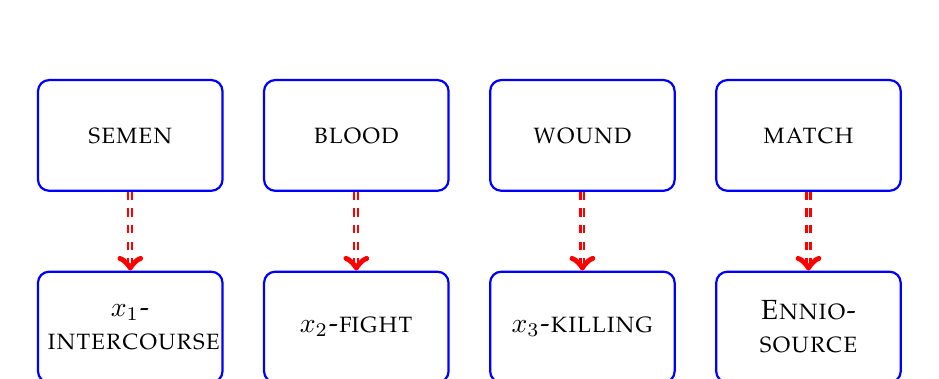
\begin{tikzpicture} 
[auto, 
block/.style ={rectangle, draw=blue, thick, 
text width=6em,align=center, rounded corners, 
minimum height=4em}, 
cloud/.style ={rectangle, draw=red, thick, 
text width=11em,align=center, rounded corners, 
minimum height=4em}, 
line/.style ={draw, thick, -latexÕ,shorten >=2pt}] 
\matrix [column sep=5mm,row sep=10mm] 
{ 
\node [block] (sem) {\textsc{semen}}; 
& 
\node [block] (bl) {\textsc{blood}}; 
&
\node [block] (wo) {\textsc{wound}};
&
\node [block] (ma) {\textsc{match}}; \\ 
% row 2 
 \node [block] (int)  {\textsc{$x_1$-intercourse}}; 
 & 
 \node [block] (f)  {\textsc{$x_2$-fight}}; 
 &  
 \node [block] (kill)  {\textsc{$x_3$-killing}}; 
 &  
\node [block] (pres)  {\textsc{Ennio-source}}; \\ 
}; 
\draw[->, red, double, dashed, thick] (sem) -- (int); 
\draw[->, red, double, dashed, thick] (bl) -- (f); 
\draw[->, red, double, dashed, thick] (wo) -- (kill); 
\draw[->, red, double, dashed, thick] (ma) -- (pres); 
\end{tikzpicture} 

\noindent
The inference from the genetic match to the hypothesis that Ennio is the 
source of the crime scene DNA was discussed earlier while examining 
the evidential strength of DNA evidence.
The acceptability of the other hypotheses
(i.e.\ intercourse; fight; killing) depends on a number 
of case-by-case details: whether the semen on the victim's body was in a quantity, location, 
and arrangement that indicate intercourse; whether the wound on the victim's body was caused by a human artifact, e.g.\ a knife, and whether this caused 
the victim's death; etc. Without dwelling on unnecessary details, let's assume 
that forensic experts, on the basis of their experience, are willing to claim that 
the hypotheses in question can be established, at least \textit{prima facie}  and until 
objections are raised by the defense. 

In order to make a unified case, the prosecutor can advance advance 
a \textit{unification hypothesis}, as follows:
%
\[ x_1=x_2=x_3=\textit{Ennio}\]
%
\noindent
The four initial hypotheses existed in isolation. They still left open the possibility that whoever had intercourse with the victim might be a different person 
from whoever fought with or killed the victim.  They still left open the possibility that different people participated in the crime. 
The unification hypothesis, instead, identifies Ennio as the (only or main) perpetrator. The unification hypothesis, together with the others, asserts that Ennio 
had sexual intercourse with the victim, fought with the victim and finally killed her with a knife. 

We now have a coherent and unifying case against the defendant Ennio.
What is the ground to assert the unification claim? A number of considerations could 
weigh in here: when examined by forensic experts, the crime traces suggest the presence of one perpetrator only; the crime could, in principle, be committed by one person only; Ennio would have had the physical force to commit the crime alone; etc. Depending on the information available, the unification hypothesis will be 
more or less strongly supported. The evidential support for the unification hypothesis cannot be traced back to any single piece of evidence. The support for the unification claim heavily
rests on holistic considerations based on cohesiveness.
Putting everything together, the prosecutor's unified case against 
Ennio can be described as follows:
%
\begin{quote}
\begin{singlespace}
The perpetrator  had or attempted to have sexual intercourse with the victim in the parking lot (which explains the perpetrator's 
semen on the victim's body); a fight ensued during which the victim was wounded (which explains the blood stains in the parking lot); finally, the perpetrator killed the woman with a knife (which explains the wounds on the victim's body) and hid her body in the woods. 
Ennio is the perpetrator: he has a matching DNA profile whose frequency is as low as 1 in 100 millon.
\end{singlespace}
\end{quote}
%



\paragraph{	Good properties of scenarios: completeness, plausibility (here??), coverage (see Pennington and Hastie)}

\paragraph{	Scenario schemes (Schank, Bex)}

\paragraph{Arguments}

\paragraph{Inference to the best explanation (Allen/Pardo?)}

\paragraph{WORRY: Confused about this one; why is it under coherence?) [Answer BV: Otherwise nothing remains here. ]}

\subsection{Probability}


\paragraph{Hierarchy of propositions (Evett et al)}


\paragraph{Combining difference pieces of evidence using probability}


\paragraph{Multiplying likelihood ratios and question of independence among difference pieces of evidence}



We first need a general account of how to 
model the \textit{combination} of two pieces of evidence E1 and E2, each supporting, with its own degree of strength, the same hypothesis H. If the strength of a single pieces of evidence $E$ depends on how much it impacts $P(H)$, the same applies to the combination of two pieces of evidence. 
Bayes' theorem shows us how the combination of E1 and E2  impacts the probability $P(H)$, as follows:
%
\[\frac{P(H| E1, E2)}{P(\neg H| E1, E2)}=\frac{P(E1\wedge E2|H)}{P(E1\wedge E2|\neg H)}\times \frac{P(H)}{P(\neg H)}.\]
%
If E1 and E2 are independent and do not influence one another, we have:
%
\[\frac{P(H| E1, E2)}{P(\neg H| E1, E2)}=\frac{P(E1|H)}{P(E1|\neg H)}\times\frac{P(E2|H)}{P(E2|\neg H)}\times \frac{P(H)}{P(\neg H)}.\]
%
\[\frac{P(H| E1, E2)}{P(\neg H| E1, E2)}= LR1\times LR2 \times \frac{P(H)}{P(\neg H)}.\]
%
Suppose, in a criminal case, DNA evidence shows that the crime traces match with defendant's 
DNA. The DNA match has a likelihood ratio, relative to hypothesis $S$, of 1,000. Another piece of evidence, independent of the DNA evidence, shows that the crime scene blood type is the same as the defendant's blood type. Suppose the likelihood ratio is now just 10. 
So, the combined evidential strength of the two pieces 
of evidence is $1,000\times 10=10,000$. This is an example of how two pieces of evidence converge  toward the 
same hypothesis.


\paragraph{This seems a largely unsolved problem for probabilistic accounts (and for the others accounts as well)}

\paragraph{The BN connection}


\section{Introduction and exclusion of the evidence}

%In many democratic countries, the trial system is designed to favor the introduction 
%of the evidence. At the same time,  certain rules exist which restrict the admissibility of the evidence for reasons such as prejudice or confusion of the issue. 
%Legal arguments in a court of law are based on the assessment of the evidence presented by both parties.  
This section illustrates the legal rules for the 
introduction and the exclusion of the evidence. An exhaustive examination of the topic cannot be undertaken here. Instead, a few 
illustrative examples, mostly taken from the federal law of the United States, will be discussed. 

\paragraph{Rules of discovery/compulsory process/evidence introduction}

%A decision to hold a defendant criminally or civilly liable must be based on the evidence presented at trial. The introduction of the evidence in a court 
%of law is a crucial aspect of the decision making process. 
The parties in a trial---plaintiff and defendant in a civil case; prosecutor and defendant in a criminal case---have an interest in presenting evidence that supports their own version of the facts, but they also have an interest 
in withholding evidence that would weaken their position. A purely adversarial trial would be one in which each party makes its best case and the decision about what evidence to introduce is entirely left to the strategizing of the parties without any regulation governing the process. The problem with this arrangement is that the divergent interests of the parties 
%in presenting or withholding evidence 
might hinder the discovery of the truth and put indigent defendants at a serious disadvantage. For example, suppose a prosecutor or plaintiff possesses evidence favoring the defendant but does not disclose it 
because of reasons of self interest. The withholding of the evidence would hinder the discovery of the truth and be unfair toward the defendant. The defendant, to be sure, might find the exculpating evidence himself but that might require extensive research and monetary disbursement on his part which an indigent might not be able to front. Therefore, legal rules about the introduction of the evidence should be in 
place to correct the imbalances of power that may arise between the parties in a trial.


Legal rules that are expected to correct  imbalances of power are the \textit{rules of discovery}. 
They regulate how the litigants should retrieve and disclose to one another the evidence in their possession. %These rules vary significantly across criminal and civil cases. 
In civil cases, discovery rules are liberal and broad. For example, rule 26(a)(1)(A)(i) of the Federal Rules of Civil Procedure 
states that a party must disclose to the other party the identities of the individuals who possess relevant information
which the party intends to use for its case or its defense (unless the information is intended for the sole impeachment purpose). %Rule 26(a)(2)(A) states that each party must disclose to the other parties 
%the identify of any expert witness the party intends to call to testify. 
This rule deals with \textit{required discovery}, but there are also rules that deal with \textit{discovery upon request}. 
Rule 26(b)(1), for example, states that any relevant evidence, both in favor and against the defendant, must be disclosed by the party who possesses it upon request.

Such broad and liberal discovery rules place defendants and plaintiffs on an equal footing insofar as 
both are under the obligation to disclose relevant information, either mandatorily or upon request by the other party. 
%Interestingly, discoverable information need not be information that can be admissible in court as evidence. %Rule 26(b)(1). 
The rationale for such broad discovery rules is to encourage the widest possible scrutiny of the facts prior to the trial so that trial by ambush 
is avoided.  Ar least in theory, the rules are supposed to correct the imbalances of power that may exist between the two litigants. A party, however,  
may abuse the rules and use them to artificially delay the proceedings or unnecessarily lengthen the litigation. To remedy this, 
the federal Rules of Civili Procedure, for example, states that discovery requests must be ``proportional to the 
needs of the case, considering the importance of the issues at stake in the action, the amount in controversy, the parties' relative access to relevant information, the parties' resources, the importance of the discovery in resolving the issues, and whether the burden or expense of the proposed discovery outweighs its likely benefit'' (Rule 26(b)(1)). Here we find a ''balancing test'' between the \textit{burden} associated with 
meeting the discovery request and its \textit{likely benefit}. It is the court that, either on its own or because of a party's motion, should weigh the costs and the likely benefits (Rule 26(b)(2)(C)(iii)). 
%It is somewhat puzzling how a court could weigh the costs and benefits even prior to knowing the information whose discovery is being requested.

But even with these restrictions in place, some commentators have argued that the current discovery rules in US Federal Courts are problematic, especially as a result of the explosion 
of electronic evidence and digital materials. Part of the problem here might be due to the fact that the party discoing the information should bear the discovery costs. 
To illustrate the extent of the problem, consider a plaintiff who is suing a hospital for malpractice and requests the defendant 
to disclose email conversations of the past ten years. Now, retrieving and disclosing this information may have staggering costs, in the order of millions of dollars, given that the number of 
email messages exchanged every day in a company is considerable. The plaintiff might make this discovery request not because there could be relevant information in the email messages, 
but simply as a mere tactic to burden the defendant or force it to settle.

We cannot address the complexity of the issues surrounding discovery rules in US Federal Courts. This above discussion, however, suggests that competing interests are at play. Introducing as much evidence as possible, both for and against the defendant, seems a worthy objective, and the discovery rules we have examined are motivated by precisely this objective. At the same time, the discovery costs can be significant should be allocated fairly among the parties. A fair allocation of the costs is not easy to determine. Should the losing party bear all the costs? Should the costs be borne by the party in a position of advantage? Should the costs be borne by the who makes the discovery request 
or by the party of fulfills the resist? Should the state bear the costs? The pure epistemic objective of collecting evidence and discovering the truth must be weighed against the pragmatic limitations 
of the system, such as its antagonist nature, the limited resources of the litigants and the needs of society at large. 

At this point, it is instructive to have a brief look at discovery rules for criminal cases in federal courts. 
In Brady v. Maryland (1963), 373 U.S. 83, 
the US Supreme Court ruled that upon request the prosecutor must 
disclose exculpatory evidence that is crucial for the defendant's case. 
The defense, by contrast, is under no such obligation.
%
%The prosecutor has no right to have evidence disclosed that would be crucial for winning the case.
%In this sense, criminal rules of discovery are typically 
%biased in favor of defendants. We can see this as part of the defendant's right to a defense, protected by the Us Constitution.
%The Federal Rules of Criminal Procedures also contains that both favor defendants and place a burden on them. 
%For example, rule 16(a)(1)(E) mandates that upon defendant's request, the prosecute must disclose ``copy or photograph books, papers, documents, data, photographs, tangible objects, buildings or places'' which the prosecutor intend to use at trial. If the prosecutor complies with the defendant's request, however, Rule 16(b)(1)(A) mandates the defendant and should return the favor, as it were, if prosecutor so wishes. 
%This does not mean that the prosecution or the defense should disclose their strategies or all the details of the case, but at least, transparent disclosure avoids what we might call `surprise evidence' and allows both parties to prepare their case as diligently as possible. 
%
Another example of the asymmetry between defense and prosecution is afforded by the compulsory process. 
The 6th Amendment to the US Constitution establishes that  ``in all criminal prosecutions, the accused shall enjoy the right ... to have compulsory process for obtaining witnesses in his favor.''  
%The compulsory process is considered a fundamental right, as fundamental as the right to a defense and the right to confront and cross-examine one's accusers in a court of law. The US Supreme Court, however, has held that this right is not limitless. In Taylor v.\ Illinois (1988), 484 U.S. 400, the Court held that a witness for the defense can be prevented from testifying if the witness testimony would conflict with other procedural rules. In the case at hand, the defense did not disclose to the prosecutor, prior to the trial, that a witness would be called to testify. Because of the failure to disclose, the trow, judge ruled that the defense had therefore no right to call the wiriness to the stand. The compulsory process was thus suspected because it conflicted with certain existing rules of discovery.  On defendant's appeal, both the Illinois Court of Appeals and the US Supreme Court sided with the trial judge.
%
The compulsory process aims at ensuring that as much evidence as possible is introduced in favor of the defendant, 
although the prosecution does not enjoy the same constitutional right to compel witnesses to testify.

The asymmetry between defense and prosecution which we find in the rules of discovery as well as the compulsory process, 
expresses a precise policy decision and makes criminal proceedings---at least in principle---tilted 
in favor of defendants. The rationales for this legal arrangement  can be numerous and cannot be examined here. 
It suffices to say that the protection of the defendant against a wrongful conviction is a core 
feature of the criminal justice system in any democratic country. A wrongful conviction, after all, will result 
 in the defendant's unjust loss of liberty or even life. In civil trials, by contrast, the stakes are not so high, 
so the asymmetry between prosecution and defense need not be so pronounced.



\paragraph{Exclusionary rules}

Let us now turn to rules for the exclusion of the evidence. In general, any relevant evidence is admissible 
unless it is deemed inadmissible on the basis of specific rules of exclusion. %, the U.S.\ Constitution, an Act of congress, or rules prescribed by 
%the U.S.\ Supreme Court. 
The Federal Rules of Evidence (abbreviated FRE) reads:
%
\begin{quote}
\begin{singlespace}
All relevant evidence is admissible, except as otherwise provided by the Constitution of the United States, by Act of Congress, by these rules, or by other rules prescribed by the Supreme Court pursuant to statutory authority. Evidence which is not relevant is not admissible. (FRE\ 402)
\end{singlespace}
\end{quote}
%

\paragraph{Relevant evidence}
What is relevant evidence? 
Rule 401 of the FRE defines it as follows:
%
\begin{quote}
\begin{singlespace}
Relevant evidence means evidence having any tendency to make the existence of any fact that is of consequence to the determination of the action more probable or less probable than it would be without the evidence. (F.R.E.\ 401)
\end{singlespace}
\end{quote}
%
It is customary to distinguish two dimensions operating in this definition: materiality and probative value \citep{Fisher2008Evidence, Mendez2008}. A piece of evidence is probative of a fact, provided the evidence makes the fact more (or less) probable than it would be in absence of the evidence. This is no different from the probabilistic characterization of 
evidential favoring, according to which a piece of evidence $E$ supports a hypothesis $H$ provided $P(E|H)> P(H)$ (SEE EARLIER SECTION OF THIS CHAPTER). 

Incidentally, note that the word `fact' can be misleading. In ordinary language, a fact is an occurrence or state of affairs that is true. If we say `that's a fact', we are referring to 
something that is---or at lest, we take to be---unquestionably true. In legal jargon, instead, a fact is sometimes understood to be a proposition 
that can be true or false. In this sense, facts at no different from hypotheses that can be true or false.

%We shall use the word 'fact' in this technical legal sense. 

Besides the probative value of a piece of evidence relative to a fact (or a hypothesis), the materiality of the evidence 
is also important. A fact is material for establishing the action or crime under examination if it is of consequence to the determination of the action or crime. Whether or not a fact is of consequence to the determination of the action or crime depends on the substantive law which determines what facts should be proven in order to establish what crimes. EXAMPLE NEEDED HERE. Also, a fact is material if it is intermediary, that is, it is a fact that if true would help prove or disprove certain elements of the crime. EXAMPLE NEEDED HERE. Finally, a fact is material if it is evidentiary. For example, it is important to know whether the witness for the prosecutor was in fact present at the time of the crime. This has little to do with what the perpetrator did or with the crime itself, but it is an evidentiary fact that is important to ascertain.  
REFERENCE MISSING. 

By combining probative value and materiality, we arrive at the following definition. A piece of evidence is relevant for establishing the commission of a 
crime if and only if the evidence is probative of a fact that is material for the crime. Relevance is a question of logic and common sense; it is not a legal question. 
There are no legal rules that prescribe the conditions under which an item of evidence is relevant or not. Logic and common should suffice here. REFERENCES HERE. EXPLAIN MORE?
If the evidence is relevant, then it must in principle be admissible unless there is an exclusionary rule that rules it inadmissible. 
So, once the question of relevance is settled, admissibility becomes a strictly legal question whose answer depends 
on the law of the particular jurisdiction. 

We shall now consider three well-established exclusionary rules 
that apply to trial proceedings in US federal courts: 
prejudice; character evidence; and hearsay. 


\paragraph{Prejudice}
To begin with, rule 403 of the FRE 
establishes that:
%
\begin{quote}
\begin{singlespace}
Although relevant, evidence may be excluded if its probative value is substantially outweighed by the danger of unfair prejudice, confusion of the issues, or misleading the jury, or by considerations of undue delay, waste of time, or needless presentation of cumulative evidence. (F.R.E.\ 403)
\end{singlespace}
\end{quote}
%
The rule requires the judge to perform a balancing test between the probative value of the evidence 
and certain negative or detrimental effects (prejudice, confusion, waste of time, etc.) that 
would be more or less likely to occur if the contested piece of evidence were to be introduced.
This is a curious rule whose standard of application is far from being 
well defined. For instance, what are the items that are intended to be balanced? 
The degree of probative value with the likelihood of prejudice, confusions, waste of time, etc.? 
Or, the degree of probative value with the degree of harm associated with prejudice, confusion, waste of time? Does the balancing 
test include all three variables at once?  REFERENCES NEEDED.

We do not hope to settle these question here. It is noteworthy, however, that the rule in question requires the judge to balance an 
epistemic value, such as the probative value of the evidence, with non-epistemic values or disvalues, 
such as prejudice, confusion and waste of time. %\footnote{To be sure, prejudice and confusion might be epistemic (dis)values.} 
%The rule states that probative value is not always enough to guarantee admissibility, and hence a balancing test between epistemic and non-epistemic dimensions 
%must be performed by the judge. The balancing-test of the two dimensions assumes that they 
%can be compared using some common metric. 
Some have questioned whether any balancing test across epistemic and non-epistemic values is at all 
possible because it would be like comparing apples and oranges \citep{taruffo09}. On the other hand, balancing tests are ubiquitous 
in the law of evidence and procedure. 
In 4th Amendment case law about (un)reasonable searches and seizures, for example, two competing goals must be reconciled. One goal is the state's need to collect evidence and the other is the citizen's 
right not to have their privacy rights violated. The Supreme Court solution, in some cases, is to adopt a balancing-test. REFERENCES NEEDED HERE. It is an interesting question on its own
whether the ``balancing strategy'' is the only, or the most appropriate strategy to undertake in case of a value conflict.

\paragraph{Character evidence}

We now turn to Rule rule 404(b) of the FRE about character evidence:
%
\begin{quote}
\begin{singlespace}
Evidence of other crimes, wrongs, or acts is not admissible to prove 
the character of a person in order to show action in conformity therewith.
(F.R.E., 404(b))
\end{singlespace}
\end{quote}
%
Character evidence concerns the previous conduct of the defendant, not the specific conduct 
under examination at trial. One reason why character evidence is considered inadmissible might be  
that it is irrelevant. Insofar as trials are \textit{not} about what the defendant did prior to the alleged crime, character evidence is irrelevant. But, excluding character 
evidence on this ground would be too drastic. There is no doubt that past offenders are more likely to reoffend than those without a criminal record REFERENCE NEEDED HERE. If this is correct, 
character evidence must count as relevant, at least insofar as the definition of relevant evidence from the FRE, rule 401, is concerned. The reason why character evidence is excluded, then, cannot be its lack of relevance. The problem with character evidence is of another sort. Although it is relevant, character evidence can have significant 
prejudicial effects on the decision making process. This is true especially in a jury trial in which the the jurors might take 
the defendant's criminal record as unduly strong evidence that the defendant did engage in criminal conduct one more time. The problem with character 
evidence, then, is that the lay jurors might exaggerate its probative value. 

It is, however, far from uncontroversial that character evidence should be excluded from trials. The exclusion of character 
is mostly a feature of the common law tradition, but even in the common law there are exceptions to the rule, %the exclusion of character evidence, 
%The legal system of countries outside the common law tradition do not have such clear exclusionary rules against character evidence. 
%Interestingly enough, even scholars in the common law tradition 
and some scholars have recently argued that character character evidence should be admissible \citep{redmayne02}.

\paragraph{Hearsay} Together with the exclusion of character evidence, the exclusion of hearsay evidence is a well-entrenched rule in the common law. Rule 802 of FRE established that hearsay evidence is 
not admissible unless provided otherwise by the FRE themselves or some other legal provision. DEFINITION OF HEARSAY. There are countless exceptions to the hearsay rule, and some of these are described in rule 803 of the FRE. EXAMPLE OF THE EXCEPTIONS. 

There are at least a couple of rationales for the exclusion of hearsay evidence. One rationale is that it is unreliable. A witness who saw the crime and can recount what she saw in court seems a more reliable source of information than a second hand-witness who can only recount what another witness told her about the crime. It is because of the more indirect chain of transmission of information that hearsay evidence might be less reliable. The more intermediaries in the chain, the more corrupt the information at the end of the chain. REFERENCES NEEDED.  Another reason why hearsay evidence is excluded is that it cannot be  scrutinized or cross examined. If witness 1 testifies in court that witness 2 told witness 1 that the defendant did so and so during the crime, the witness that should be cross examined is witness 2, and instead the witness who is testifying in court is witness 1. This setting undermines the right of defendants to confront their accusers and cross examine them. REFERENCES. MORE EXPLANATION NEEDED HERE. 









\paragraph{Exclusionary rules, free proof, rules of weight}

THIS PARAGRAPH WILL DISCUSS ALTERNATIVES TO THE SYSTEM OF ADMISSIBILITY RULES. ONE ALTERNATIVE IS FREE PROOF, WHICH MEASN TO INTRODUCE AS MUCH EVIDENCE AS POSSIBLE WITHOUT ANY RULE OF EXCLUSION OR VIRTUALLY NO RULE OF EXCLUSION. THE OTHER ALTERNATIVE IS HAVING RULES OF WEIGHT, RULES THAT DETERMINE HOW THE EVIDENCE SHOULD BE WEIGHTED AND ASSESSED. THE SYSTEM OF ADMISSIBILITY RULE SITS SOMEWHERE IN THE MIDDLE.






\section{When can we convict?}


%\subsection{Beyond a reasonable doubt}

Once all the evidence has been introduced at trial, examined and cross-examined, it comes a time when the fact-finders---either a trained judge or the jurors themselves---have 
to make a decision. Convict or acquit? The decision must be based on the evidence presented, and not on human sympathy or hatred, and it must be based 
on the law governing the case. This still leaves open an important question. What decision criterion governs the decision? This criterion, in criminal trials, is known as the \textit{beyond a reasonable doubt} standard and it is adopted in many countries even outside the common law countries. MORE EXPLANATION HERE (TALK ABOUT FRANCE GERMANY ITALY SPAIN) 
If the fact-finders are persuaded of the defendant's guilt beyond a reasonable doubt, they should convict, or else they should acquit. This rises a host of difficult questions. What does  it mean to establish guilt beyond a reasonable doubt? When is a doubt reasonable or unreasonable? Can the standard be given a more precise meaning and characterization? We can only begin to scratch at the surface of these questions and point the reader toward existing literature. 
  
  \paragraph{Informal clarifications}
  Explications of when a doubt is reasonable or unreasonable abound. In Commonwealth v.\ Massachusetts Webster (1850), 
proof beyond a reasonable doubt is equated to `reasonable and moral certainty' (295, 59 Mass., 320).  Another paraphrase is that proof beyond a reasonable doubt is such that `a reasonable person would not hesitate to act upon it in the most important of his own affairs,' or again, proof beyond a reasonable doubt must cause `an abiding conviction in the minds of the jurors.' These paraphrases might not be that unhelpful, and if so, the U.S.\ Supreme Court is quite right when it says that `attempts to explain the term ``reasonable doubt'' do not result in making it any clearer' (Holland v.\ United States (1954), 348 U.S. 121, 140). 

%Nevertheless, we still have a grasp of what the criminal standard is supposed to \textit{do}, though we cannot articulate what it is supposed to \textit{mean}. 

Another strategy for clarifying proof beyond a reasonable doubt is to identify 
certain constraints that the standard should satisfy, avoiding the trouble 
of proving a precise definition. Following this strategy, the Supreme Court of Canada in R.\ v.\ Lifchus (1997) 
listed some platitudes which are worth stating:

\begin{quote}
(-) the standard of proof beyond a reasonable 
doubt is inextricably intertwined with that  
principle fundamental to all criminal trials, 
the presumption of innocence;

(-) the burden of proof rests on the prosecution 
throughout the trial and never shifts to the
accused; 

(-) a reasonable doubt is not a doubt based upon 
sympathy or prejudice; 
rather, it is based upon reason and common sense;

(-) it is logically connected to the evidence or  
absence of evidence; 
 
(-) it does not involve proof to an absolute certainty; it is not proof beyond any doubt nor is 
it an imaginary or frivolous doubt;  and

R.\ v.\ Lifchus (1997) at 335.
\end{quote}

\noindent
Most would find the Court's remarks unobjectionable. The  Court did not only explicate when a doubt is `reasonable,' 
but it also explicitly linked the criminal standard to other related notions, such as the presumption of innocence, the burden of proof, the presence and absence of evidence, 
reason and common sense. These connections are important and help us see the role that the standard proof beyond a reasonable doubt plays in the criminal trial. 
%The first two platitudes emphasize that it is the prosecutor that 
%should establish guilt and not the defense that should innocence. 


\paragraph{Probability-based account}

For those who seek a more analytic characterization of the standard, 
these informal clarifications might be unsatisfactory. Legal scholars have tried to give more analytic characterizations 
and we shall consider three such attempts.  In the existing literature, one prominent view is legal probabilism. It is the view that establishing guilt beyond a reasonable doubt means to establish that the defendant's \textit{probability of guilt}, given the total evidence presented at trial, meets a threshold, say, 0.99 or 0.999  \citep{Kaplan1968Decision, Kaye1999Clarifying-the-, Tillers2007}. Consequently, a doubt would be reasonable or unreasonable depending on a measurable probability.  

This definition is simple, crisp and elegant, but a too literal interpretation of it is obviously problematic.  If a probabilistic threshold is understood as a criterion which the fact-finders should mechanically apply whenever they confront the decision to convict or acquit, two difficulties arise. The first difficulty is that assigning a probability value to guilt itself might not be feasible. This difficulty, however,  can be sidestepped if we understand legal probabilism less mechanistically.  The legal probabilists can defend their proposal by conceding that they are not offering a recipe that should be directly implementable in court. Assigning probabilities to propositions, they could say, is an idealized process, a regulative ideal which can improve trial proceedings. In this spirit, setting a probabilistic criterion for criminal convictions would only be a way to theorize about the meaning and function of the criminal standard of proof. REFERENCE HERE. 

The second difficulty is that it is not clear where, exactly, the threshold should be placed: is it 0.99, 0.89, 0.899, 0.999, or what? The difficult here is not so much with identifying a precise numerical value. 
After all, a range of acceptable values instead of a precise threshold could still be used. The problem here is rather, where to place the bar, whether the bar corresponds to a precise value or an interval of acceptable values? IN response to this question, David Kaplan used a relative assessment 
of the disutilities associated with convicting an innocent, $D_i$, and with acquitting a guilty defendant, $D_g$.  
Suppose the probability of guilt and innocence equals $P_g$ and $P_i$ such that $P_g = 1 - P_i$. 
To convict---Kaplan suggests---the jury must be believe that 

\vspace{2mm}

$P_g D_g > (1-P_g) D_i$.

\vspace{2mm}
\noindent
The inequality represents a situation in which the expected disutility resulting from acquitting a guilty defendant is larger than the disutility resulting from 
convicting an innocent defendant. So, given the inevitable possibility of error, such a situation would be one in which 
convicting is less harmful than acquitting, so that conviction is justified. As one can see, this is an application of the more general statistical decision theory based on maximization of expected utility or the minimization of expected loss. REFERENCES HERE. 

The inequality holds only if $P_g$ reaches a certain value. 
From the inequality, by algebra, we have

\vspace{2mm}
$\frac{P_g}{1- P_g} > \frac{D_i}{D_g}$.

\vspace{2mm}
\noindent
This formula gives a precise indication of how high the probability 
of guilt must be to justify a guilty verdict, relative to the ratio between $D_i$ and $D_g$. If we consider that
the disutility of convicting an innocent is as harmful as the disutility of acquitting an innocent, 
i.e., $D_g=D_i$---as it might be the case in a civil case---, the lower bound for $P_g$ must be at least $\frac{1} {2}$. 
If, instead,we think that $\frac{D_i}{D_g}=\frac{9}{1}$---as it might be more appropriate in a criminal 
case---, the lower bound for $P_g$ must be at least $0.9$. More complicated models are also possible, 
but the basic idea is that the probability required for a conviction will be a function of weighing certain social and 
economic costs that would result from erroneous decisions. 



\paragraph{Scenario-based account}


Some scholars suggested that we should elaborate a 
theory of legal reasoning which departs from the 
probabilistc approach and which does not ignore trial procedures broadly construed
\citep{cohen77, nesson79, Thomson86, Walton2002, Stein05, Pardo2008Judicial-Proof-, ho08, Haack2011Legal-Probabili}.
The key notion here seems to be plausibility rather than probability.
Ronald \cite{Allen2010No-Plausible-Al} recently suggested that that 
`[no] plausible alternative to a plausible story of guilt [should be] the rule of decision in criminal cases'
and that `[i]n criminal cases, fact finders find guilt if there is a plausible story of guilt and 
no plausible story of innocence; otherwise, they find innocence.'

The plausibility-based approach is appealing, but the obvious problem is that the notion of a `plausible story' or of a `plausible alternative to a plausible story' is wholly under-defined. 
SAY MORE HERE
Still, if the notion of plausibility is hard to define precisely, it seems closer to how jurors actually reason in trial proceedings, whereas the notion of probability, despite its 
mathematical underpinnings, is hard to relate to actual trial proceedings: jurors do not naturally quantify guilt, and it is difficult to quantify it 
even if we wanted to. We face a trade-off: probability is a formally developed notion, but it is 
removed from trial proceedings and common-sense reasoning; plausibility 
lacks a well-established theory, but it is closer to trial practice. 


\paragraph{Argumentation-based account}


\section{Summary and conclusion}

%\bibliographystyle{spbasic}
\bibliographystyle{plainnat}	
\bibliography{dissertation}






\end{document}

